\documentclass{ctexbeamer}
% \documentclass[handout]{ctexbeamer}
% \documentclass{beamer}
\usetheme{Montpellier}
\usepackage{graphicx}
\usepackage{beamerbasetitle}
\usepackage{listing}
\graphicspath{ {./images/} }
\usepackage{multicol}
\usefonttheme[onlymath]{serif}
\usepackage{hyperref}
\usepackage[backend=bibtex,sorting=none]{biblatex}
\nocite{*}
\addbibresource{./ref/ref.bib} 
\setbeamerfont{footnote}{size=\tiny}

\usepackage{minted}
\usepackage{ulem}

\usepackage[svgnames]{xcolor}
\usepackage{tcolorbox}
\newtcolorbox{notice}[1][]{colback=yellow!10!white, colframe=yellow!50!black, title=#1}

% Define Light Gray
\definecolor{LightGray}{gray}{0.9}
\setminted{autogobble = true, baselinestretch = 0.9, beameroverlays = on, escapeinside=||}

\setminted{linenos=true}

\hypersetup{
  colorlinks,
  allcolors=.,
  urlcolor=blue,
}
\definecolor{PKUblack}{rgb}{0, 0, 0} % UBC Blue (primary)
\definecolor{PKUred}{HTML}{b23333} % UBC Grey (secondary)

\title{Tutorial 2: Python 基础类型与运算}
\author{方嘉聪}
\institute{jiacong\_fang@stu.pku.edu.cn}
\date{2025年3月6日}

% \begin{minted}[bgcolor=LightGray]{python}
%     >>> from math import pi
%     >>> pi**2
%     9.869604401089358
%     >>>
% \end{minted}

\begin{document}
    % \large
    \begin{frame}
        \titlepage
    \end{frame}

    \AtBeginSection[]
    {
        \begin{frame}<beamer>
            \frametitle{目录}
            \tableofcontents[currentsection]
        \end{frame}
    }
    \section{课程安排}
    \subsection{第一次作业}
    \begin{frame}[fragile]  
        \frametitle{作业安排}     
        作业一已经发布: 
        \begin{itemize}
            \item 主要内容: 基础语法, 包含0304与0311两次课的内容;
            \item 其中7-8题与字符串基本操作与格式化输出相关;
            \item \underline{\textcolor{red}{截止时间: 2025-03-20 17:00:00}}
        \end{itemize}
        \vspace{2em}
        请大家确认已经加入了Openjudge. \href{http://csc6.openjudge.cn}{http://csc6.openjudge.cn}
        \vspace{1em}
        
        如果还没有加入请按照教学网上的教程及时加入, 并将用户名改为 \underline{学号 + 姓名}.
    \end{frame}

    \section{Python 环境介绍}
        \subsection{命令行交互模式}
        \begin{frame}
            \frametitle{Python 交互模式}
            Python的命令行交互模式(REPL: Read-Eval-Print Loop)是一个\textcolor{red}{即问即答}的Python环境. 

            \textcolor{blue}{优势: 及时反馈, 便于学习, 不用额外创建文件}
            \begin{figure}[htpb]
                \centering
                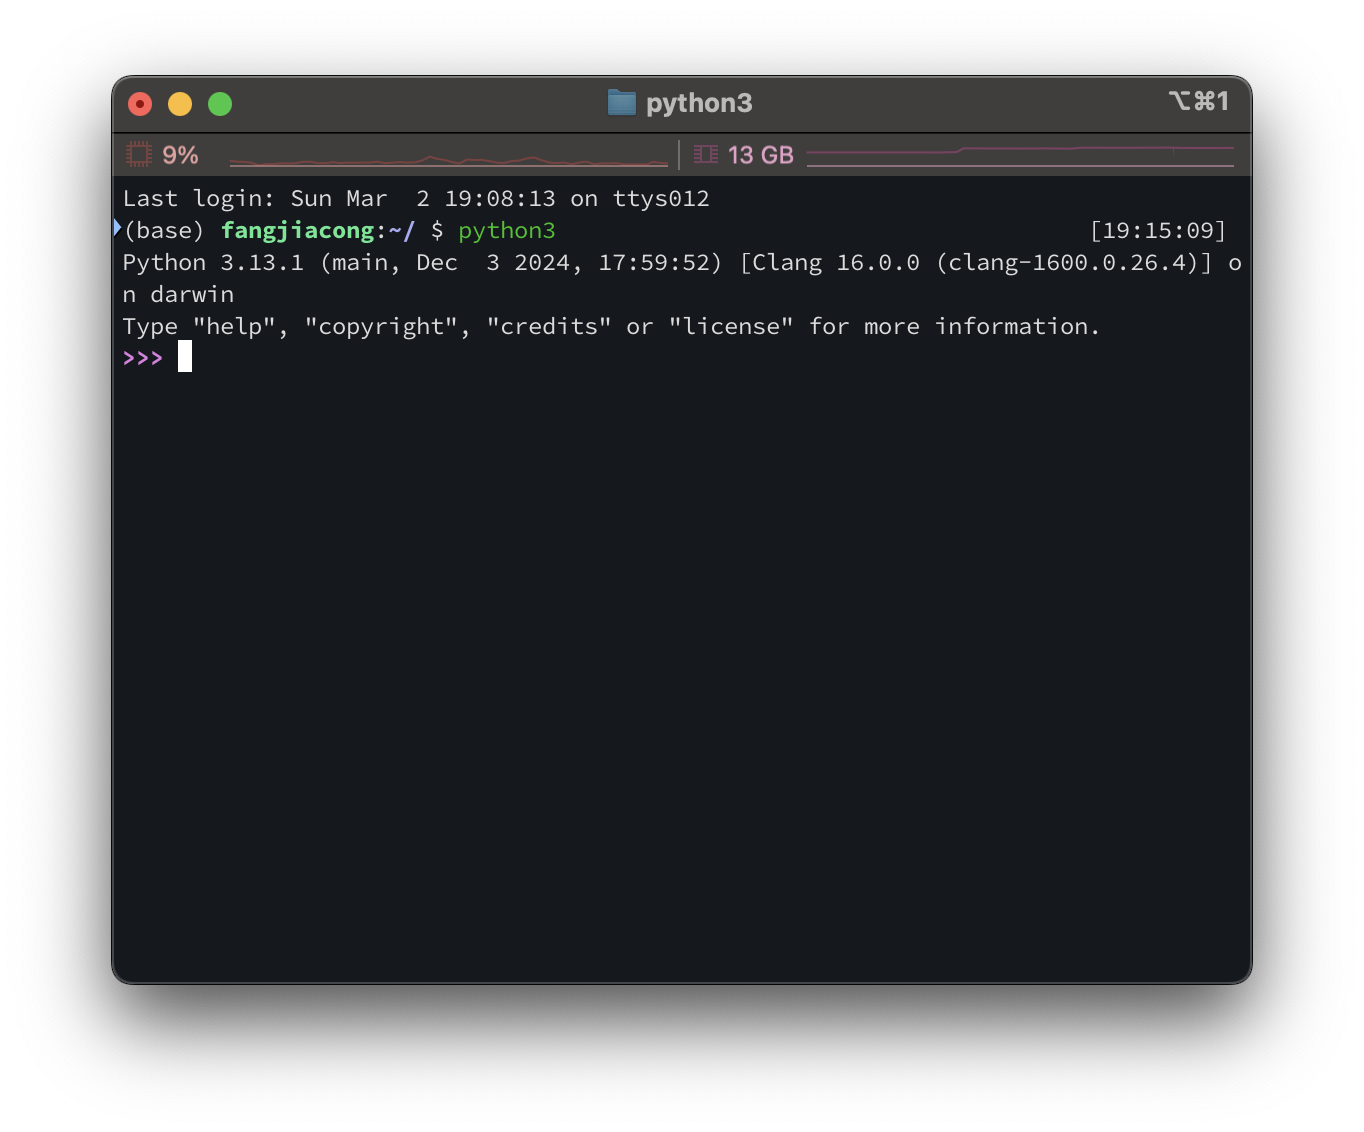
\includegraphics[width=0.7\textwidth]{./images/terminal.png}
            \end{figure}
        \end{frame}

        \begin{frame}[fragile]
            \frametitle{Python 交互模式(Cont.)}
            如何使用? Demo Here.
            \begin{enumerate}
                \item \textcolor{red}{打开终端}:
                \begin{itemize}
                    \item Windows: 按 \texttt{Win + R}, 输入 \texttt{cmd} 回车;
                    \item MacOS: 搜索 \texttt{Terminal} app, 并打开.
                \end{itemize}  
                \item \textcolor{red}{启动Python}: 
                \begin{itemize}
                    \item Windows: 输入 \texttt{python} 回车;
                    \item MacOS: 输入 \texttt{python3} 回车.
                \end{itemize}
                \item 如果启动成功,则会弹出来一系列的版本信息,然后看到下面这种符号,意味着 python 正
                在等待你的输入。
            \end{enumerate}
            \begin{minted}[bgcolor=LightGray]{python}
                Python 3.13.1 .... # 后面是一堆版本信息
                >>> 
            \end{minted}
        \end{frame}

        \begin{frame}[fragile]
            \frametitle{Python 交互模式(Cont.)}
            让我们来看一些小练习 (Python 是最好用的内置计算器!)
            \begin{minted}[bgcolor=LightGray]{python}
                >>> 2025
                ?
                >>> 2 + 2025
                ?
                >>> 2 ** 10 + 10 ** 3  # ** 表示乘方
                ?
                >>> 7 / 3
                ?
                >>> 7 // 3
                ?
                >>> 
            \end{minted}
        \end{frame}
        
        \subsection{Jupyter Notebook}
        \begin{frame}[fragile]
            \frametitle{Jupyter Notebook}
            \textcolor{red}{\textbf{Jupyter Notebook}} 是\sout{一个开源的交互式编程环境}(一个可以实时跑Python代码的``Word''), 可以方便的将代码、文本、图片和可视化内容整合在一个文档中,具体来说
            \begin{enumerate}
                \item \textcolor{red}{交互编程}:你可以逐行或逐段运行代码,且立即查看结果
                \item \textcolor{red}{笔记与代码结合}:你可以在代码旁边添加注释、说明和公式(支持 Markdown)
                \item \textcolor{red}{教学与学习}:在上机课上我们有时将使用其展示代码运行
            \end{enumerate}
            \vspace{1em} \pause
            \begin{itemize}
                \item (推荐) VS Code 中的配置参考 \underline{教学网-上机资料} 或\href{https://empty-car-8ce.notion.site/Python-VS-Code-2025-2-19fc19e4eddc809ca536c937ebfe9e6b#19fc19e4eddc80849d9bca946e704150}{该教程}.
                \item PyCharm 需要使用 Professional/Education 版本, 可以在 \href{https://www.jetbrains.com/community/education/#students}{官网} 申请 Educational License.
            \end{itemize}

        \end{frame}

        \subsection{文本编辑器/IDE}
        \begin{frame}
            \frametitle{文本编辑器/IDE}
            \textbf{代码编辑器}和\textbf{集成开发环境(IDE)}类似于 ``Word'' 或 ``备忘录'', 但是专门用于编写代码.
            \vspace{1em}
            \begin{itemize}
                \item \href{https://www.vim.org/download.php}{Vim/NeoVim}:轻量级编辑器,适合高手,但学习曲线较陡。
                \item PyCharm: 专业的Python IDE, 功能全面, 但占用内存较大。
                \item VS Code: 轻量级编辑器,丰富插件, 支持多种语言。
                \item \textbf{记事本/文本编辑器}:虽然可以用,但缺乏代码编辑的专用功能,效率较低。
            \end{itemize}
            \vspace{1em}\pause
            \begin{notice}
                注: 编辑器本身并不运行代码, 而会将代码``发送''给Python解释器(Python Kernel/Laucher)执行.
            \end{notice}
        \end{frame}

    \section{数据类型与数据运算}
    \subsection{变量的赋值与使用}
    \begin{frame}
        \frametitle{变量的存储}
        在我们写下 \mintinline{python}|a = 3| 时,发生了什么? \pause
        \begin{enumerate}
            \item 在内存中开辟一块空间,存储 \mintinline{python}|3|。 \textcolor{red}{我们把 \mintinline{python}|3| 称为值/对象。}
            \item 给 \mintinline{python}|3| 这个内存空间起一个名字 \mintinline{python}|a|。 \textcolor{red}{我们把 \mintinline{python}|a| 称为变量。}
        \end{enumerate}
        \pause\vspace{2em}
        直观上理解: 
        \begin{itemize}
            \item 把内存想象成我们现在在的房间,里面有很多盒子,
            \item 进行 \mintinline{python}|a = 3| 操作,就是找到一个空盒子,把 \mintinline{python}|3| 放进去,
            \item 然后往盒子上贴一个标签 \mintinline{python}|a|,
            \item 以后我们就可以通过 \mintinline{python}|a| 来找到这个盒子。
        \end{itemize}
    \end{frame}

    \begin{frame}[fragile]
        \frametitle{变量的被赋值和使用}
        以下面这段简单代码为例:
        \begin{minted}[bgcolor=LightGray]{python}
            a = 3   # a 首次被赋值 => 定义
            b = a   # a 被引用而后赋值给 b
            a = 4   # a 被重新赋值
        \end{minted}

        \begin{enumerate}
            \item \textcolor{blue}{赋值}: 变量在 = 左边是 \underline{被赋值}.  \textcolor{red}{标签 \mintinline{python}|a| 贴在 \mintinline{python}|3| 的盒子上。} 
            \item \textcolor{blue}{定义}: 变量首次被赋值称为\underline{被定义}, \textcolor{red}{先给 \mintinline{python}|3| 找一个盒子, 然后贴上标签 \mintinline{python}|a|。} 
            \item \textcolor{blue}{引用}: 变量在 = 右边, 参与表达式运算, 被函数调用时 \underline{被引用}. \textcolor{red}{通过标签 \mintinline{python}|a| 找到 \mintinline{python}|3| 的盒子, 再进行函数调用/表达式运算/赋值。} 
        \end{enumerate}
    \end{frame}
    \begin{frame}[fragile]
        \frametitle{变量的被赋值和使用}
        \begin{minted}[bgcolor=LightGray]{python}
            a = 3   # a 首次被赋值 => 定义
            b = a   # a 被引用而后赋值给 b
            a = 4   # a 被重新赋值
        \end{minted}

        \begin{enumerate}
            \item \textcolor{blue}{赋值}: 变量在 = 左边是 \underline{被赋值}.  \textcolor{red}{标签 \mintinline{python}|a| 贴在 \mintinline{python}|3| 的盒子上。} \pause
            \item \textcolor{blue}{定义}: 变量首次被赋值称为\underline{被定义}, \textcolor{red}{先给 \mintinline{python}|3| 找一个盒子, 然后贴上标签 \mintinline{python}|a|。}  \pause
            \item \textcolor{blue}{引用}: 变量在 = 右边, 参与表达式运算, 被函数调用时 \underline{被引用}. \textcolor{red}{通过标签 \mintinline{python}|a| 找到 \mintinline{python}|3| 的盒子, 再进行函数调用/表达式运算/赋值。} 
        \end{enumerate}
        \begin{notice}
            \textcolor{red}{注意:} 变量的使用遵循 \underline{先定义后使用} 的原则, 必须先赋值才能引用,否则报错 \mintinline{python}|NameError|
        \end{notice}
    \end{frame}

    \subsection{数据类型与运算}
    \begin{frame}[fragile]
        \frametitle{基本运算}
        \begin{center}
            \Large Demo Here. \\
            (Refer to the attached Jupyter Notebook)
        \end{center}
    \end{frame}

    \subsection{常见报错及处理}
    \begin{frame}
        \frametitle{Python 常见报错}
        \begin{enumerate}
            \item<1-> \only<1>{\textcolor{blue}}{\textbf{SyntaxError}: invalid syntax. 语法错误.}
            \begin{itemize}
                \item 为括号、引号等未成对出现. 输入了非法字符(如中文标点).
                \item 在 \mintinline{python}|if|, \mintinline{python}|for|, \mintinline{python}|while| 等语句后忘记加 \mintinline{python}|:|.
            \end{itemize}
            \item<2-> \only<2>{\textcolor{blue}}{\textbf{IndentationError}: unexpected indent. 缩进错误.}
            \begin{itemize}
                \item 代码块内部的缩进不一致. $\to$ 不要将空格与制表符混用.
            \end{itemize} 
            \item<3-> \only<3>{\textcolor{blue}}{\textbf{NameError}: name '...' is not defined. 变量未定义.}
            \begin{itemize}
                \item 变量未被赋值, 未定义就被引用.
            \end{itemize} 
            \item<4-> \only<4>{\textcolor{blue}}{\textbf{TypeError}: unsupported operand type(s) for ...}
            \begin{itemize}
                \item 不同类型的数据进行了不支持的运算. 例如 \mintinline{python}|'str' + 1|.
            \end{itemize}
            \item<5-> \only<5>{\textcolor{blue}}{\textbf{ZeroDivisionError}: division by zero. 除零错误.}
            \begin{itemize}
                \item 除数为零. 例如 \mintinline{python}|1 / 0|.
            \end{itemize}
            \item<6-> More errors will be discussed in the future. \textcolor{red}{Google it!}
        \end{enumerate}
    \end{frame}

        \begin{frame}
            \frametitle{Openjudge 评测结果}
            \begin{figure}
                \centering
                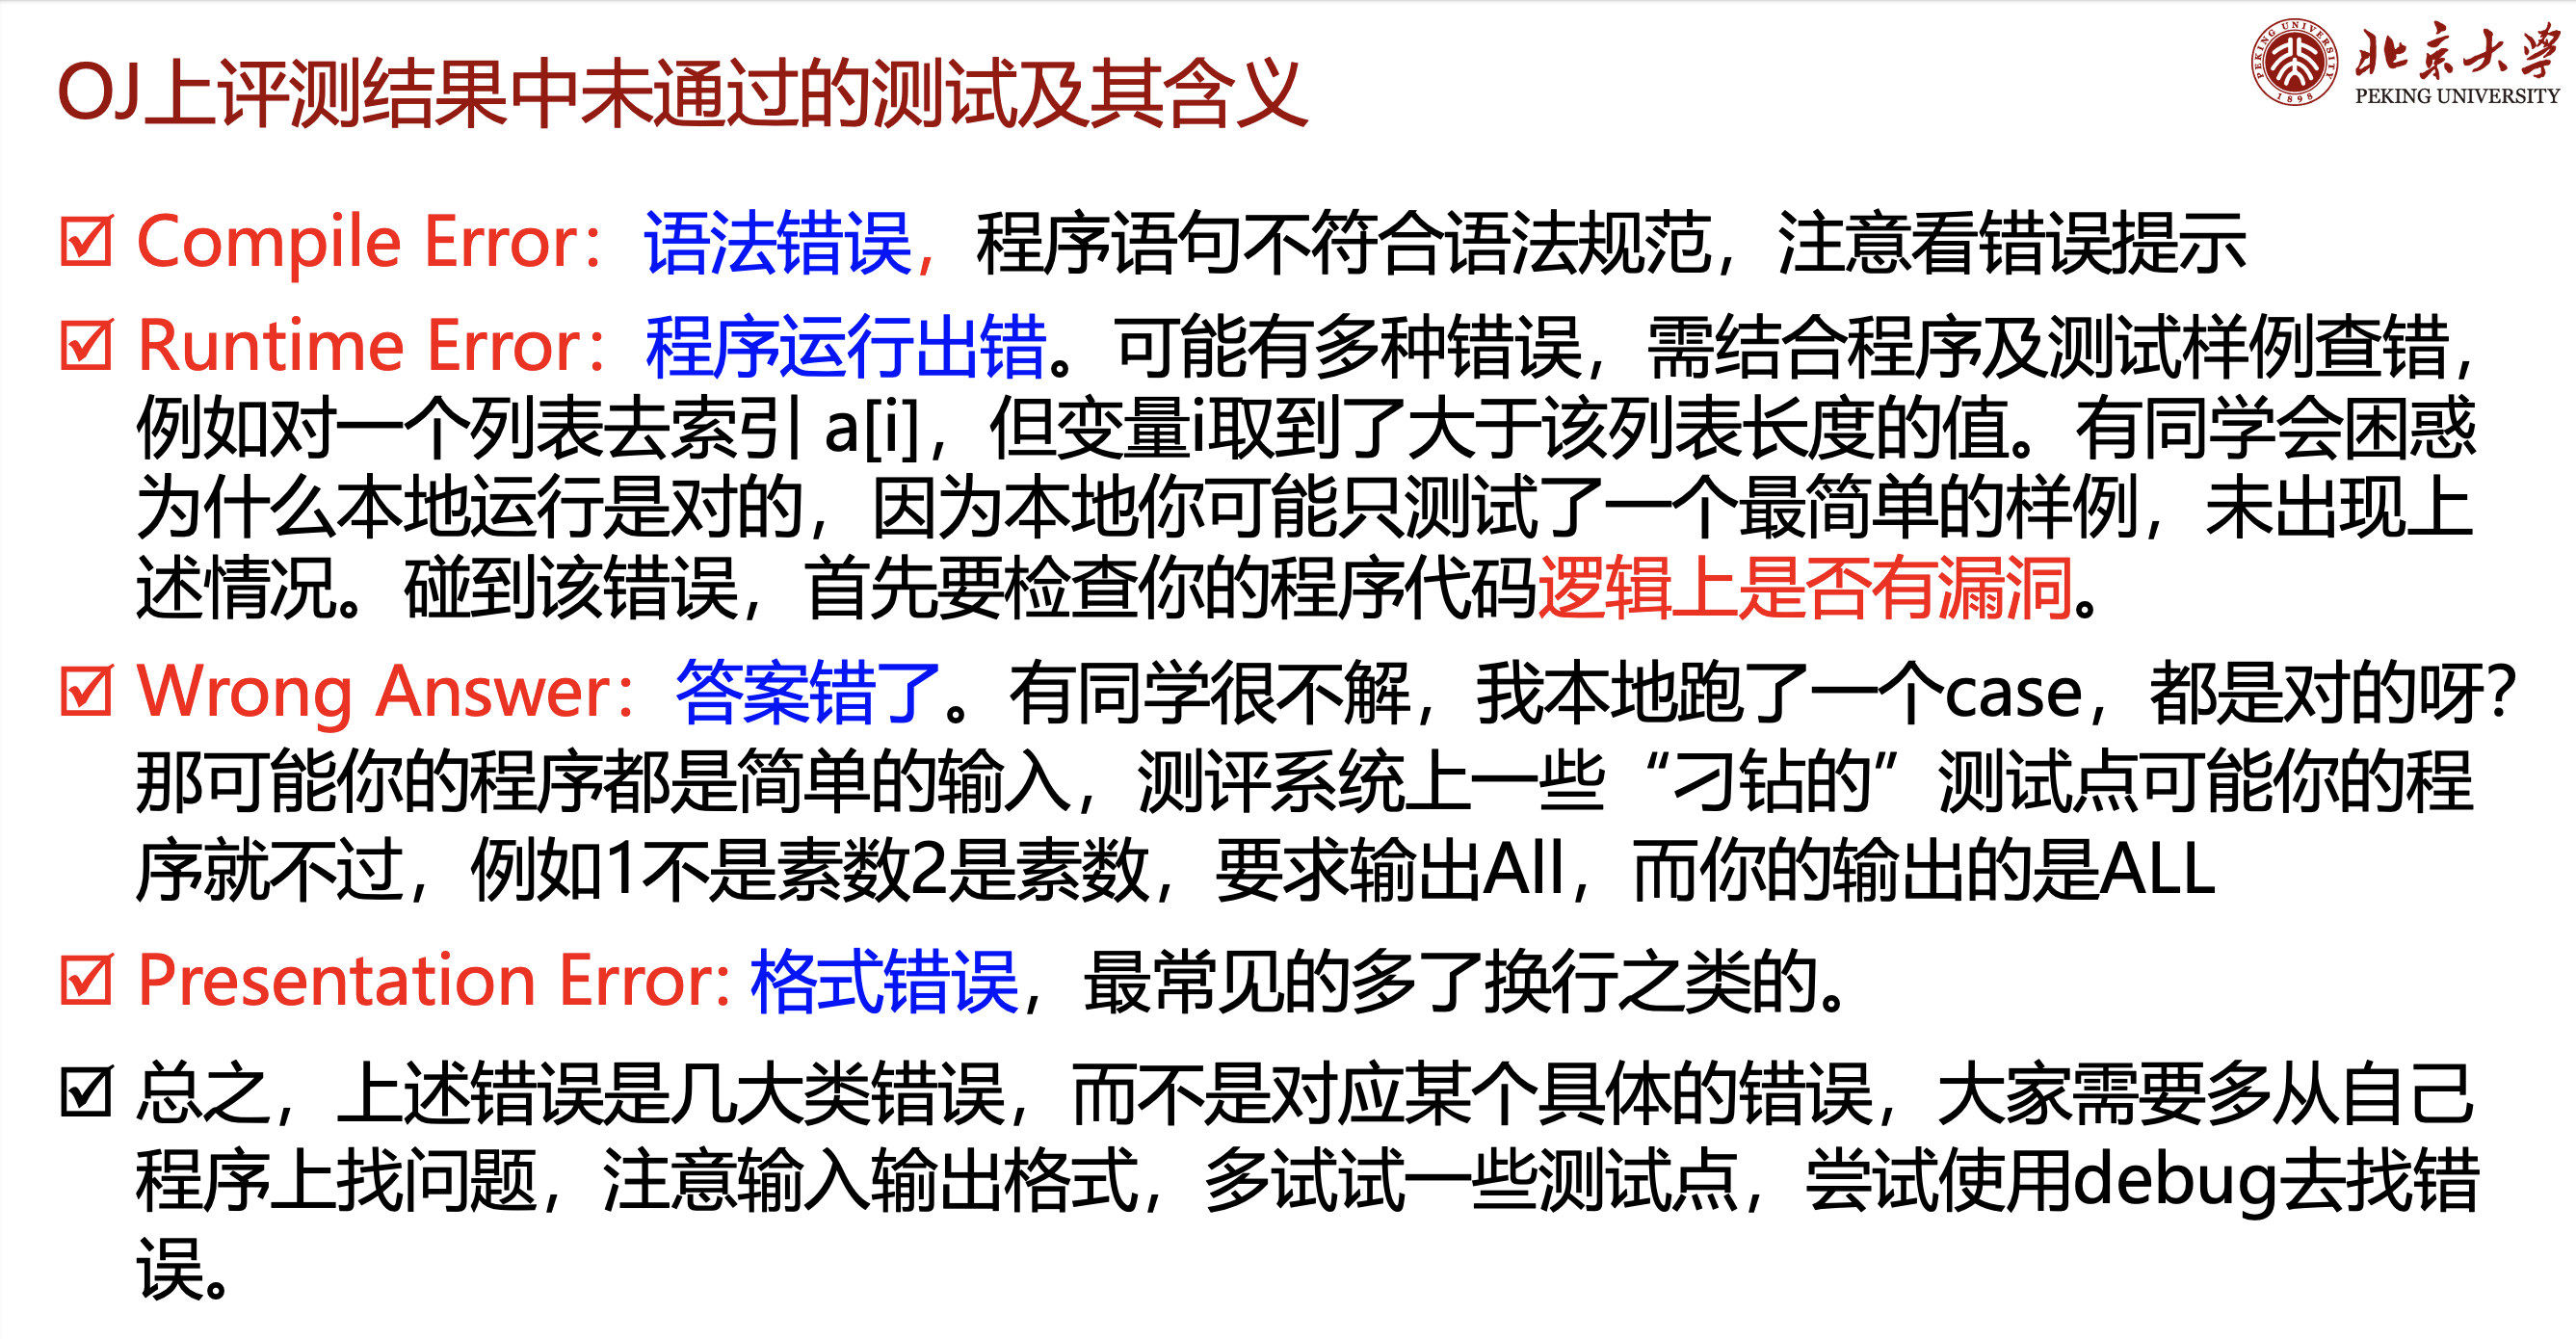
\includegraphics[width=1\textwidth]{./images/openjudge.png}
            \end{figure}
        \end{frame}

        \subsection{推荐资源}
        \begin{frame}
            \begin{itemize}
                \item 在线的 Python 代码可视化工具: \href{https://pythontutor.com/python-compiler.html}{Python Tutor}
            \end{itemize}
            \begin{figure}
                \centering
                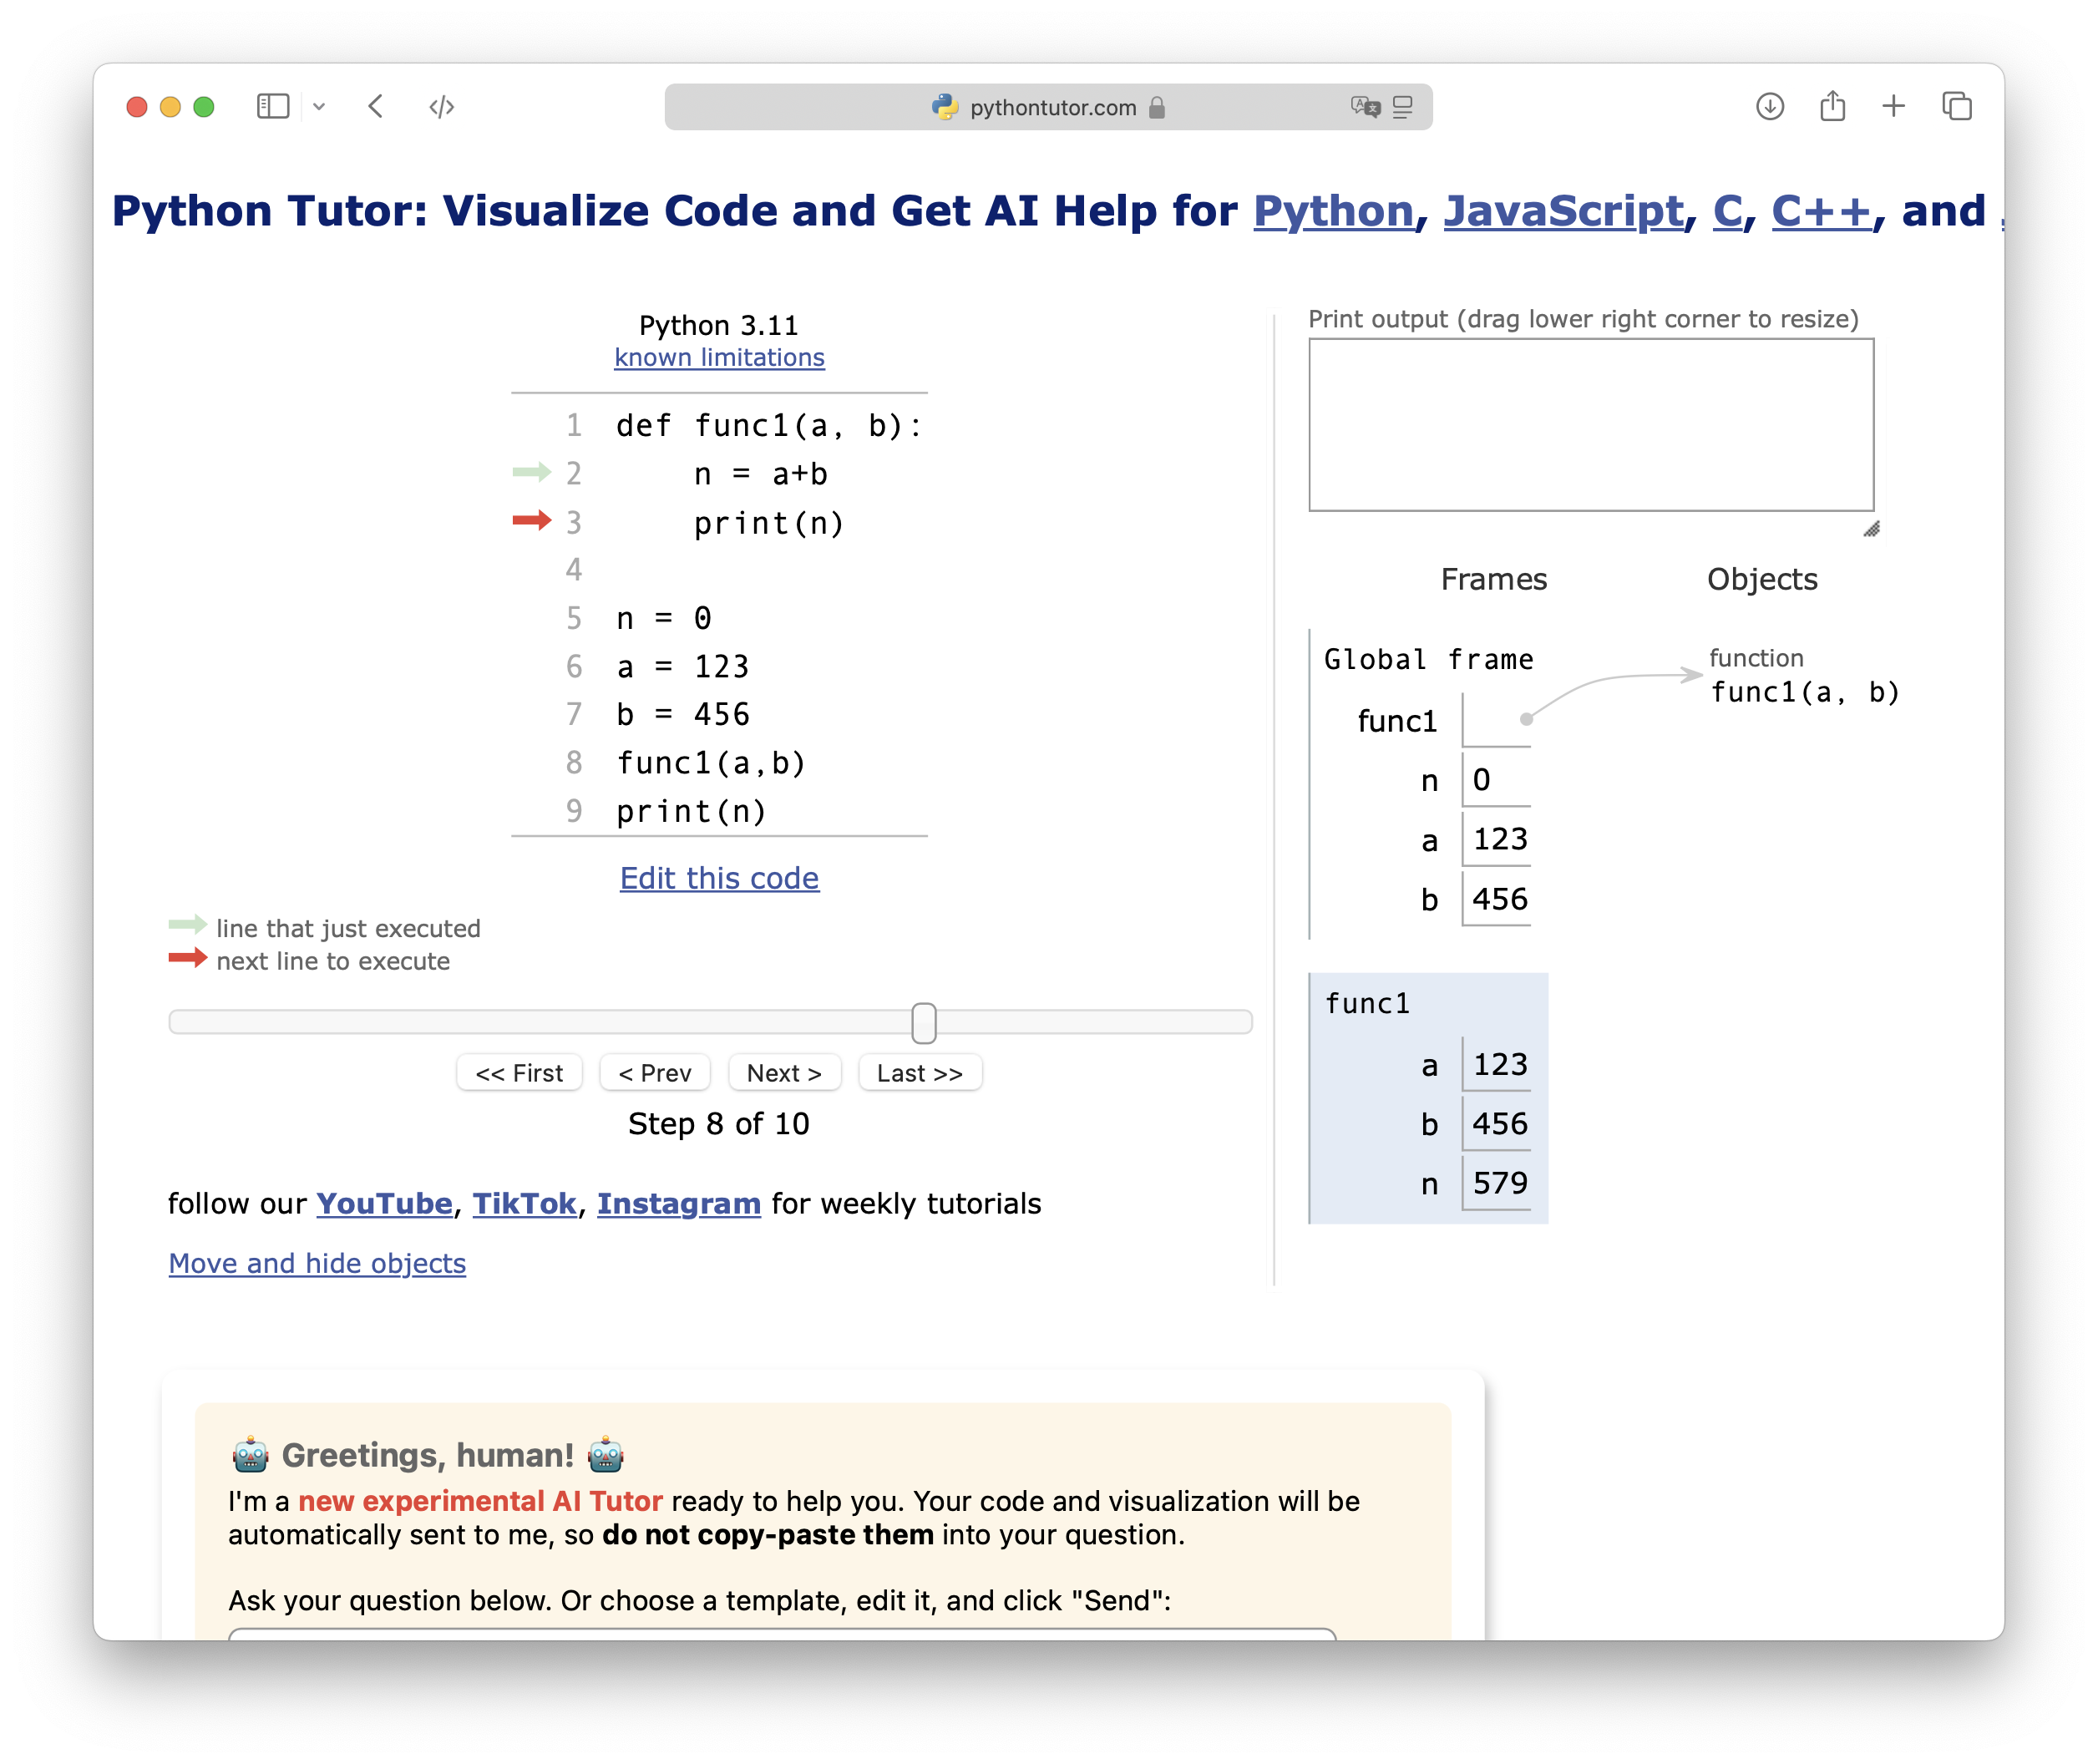
\includegraphics[width=0.75\textwidth]{./images/pythontutor.png}
            \end{figure}
        \end{frame}
        
        \begin{frame}
            \frametitle{推荐资源}   
            以下是一些有用的资源:
            \begin{itemize}
                \item 在线的 Python 代码可视化工具: \href{https://pythontutor.com/python-compiler.html}{Python Tutor}
                \item Python课程: UC Berkely CS61A \href{https://cs61a.org}{https://cs61a.org}
                \item Textbook: Composing Programs \href{https://www.composingprograms.com}{https://www.composingprograms.com}, \href{https://composingprograms.netlify.app}{社区中文版}            
                \item Markdown 官方教程: \href{https://markdown.com.cn}{https://markdown.com.cn}
            \end{itemize}
            \vspace{1em}
            个人建议: \underline{多与Python交互, 独立思考, 练习与交流}.

            \begin{itemize}
                \item \textcolor{red}{\textbf{Google and Bing are your friends.}} \sout{(Baidu)}
                \item 线上提问时请描述清楚问题, 已经做了哪些尝试. 
                \item \textcolor{red}{截图} + \textcolor{red}{代码} + \textcolor{red}{报错信息}.
            \end{itemize}
        \end{frame}
    
    % Thanks Page
    \begin{frame}
        \begin{figure}
            \centering
            
\includegraphics[width=0.4\textwidth]{./images/qrcode.jpg}
        \end{figure}
        \begin{center}
            \Large That's all for today!
        \end{center}
        \begin{center}
            My next tutorial will be on \textcolor{red}{\textbf{March 27th}}, and will cover:

            \vspace{1em}
            程序调试, 大语言模型辅助程序设计, 函数与枚举遍历算法.
        \end{center}
    \end{frame}
\end{document}